\documentclass[aps,pre,twocolumn,superscriptaddress,nofootinbib,floatfix]{revtex4-2}

\usepackage[utf8]{inputenc}
\usepackage[T1]{fontenc}
\usepackage{lmodern}
\usepackage[brazil]{babel}
\usepackage{graphicx}
\usepackage{amsmath,amssymb}
\usepackage{bm}
\usepackage{siunitx}
\sisetup{output-decimal-marker={,}}
\usepackage{booktabs}
\usepackage{subcaption}
\usepackage{tikz}
\usepackage[hidelinks]{hyperref}

\graphicspath{{figures/}}
\newcommand{\vect}[1]{\bm{#1}}
\newcommand{\uv}[1]{\hat{\bm{#1}}}
\newcommand{\avg}[1]{\left\langle #1 \right\rangle}

\newtheorem{lema}{Lema}

\raggedbottom
\begin{document}

\renewcommand{\figurename}{Fig.}
\renewcommand{\tablename}{Tabela}

\title{Dinâmica de voo de um bumerangue de papel:\\ teoria do elemento de pá, precessão giroscópica e a órbita sincronizada}

\author{Gabriel Bassi}
\affiliation{Equipe Brasil, International Young Physicists' Tournament (IYPT) 2025}


\begin{abstract}
Um bumerangue que retorna pode ser dobrado a partir de uma única folha de papel. Investigamos como o seu voo depende da geometria, das velocidades iniciais de translação e de rotação e da inclinação lateral no lançamento. O retorno resulta da sustentação assimétrica entre as asas que avançam e as que recuam, que gera um momento perpendicular ao momento angular de rotação e, portanto, uma precessão giroscópica do plano do bumerangue. Calculamos a sustentação e o momento de rolamento pela teoria do elemento de pá, usando uma identidade harmônica discreta que mostra que, para $n\geq3$ asas, a sustentação é instantaneamente constante, e descrevemos a precessão do eixo de rotação pelo mapa exponencial de $SO(3)$ (fórmula de Rodrigues). As equações de movimento admitem uma solução exata, a \emph{órbita sincronizada}, em que o plano do bumerangue e a velocidade giram juntos. Ela exige uma razão de avanço universal $\mu^\ast=\sqrt{2/3}$ e tem raio $\varrho^\ast=6I/(\rho C_L nCR^3)$, independente da velocidade de lançamento. Para uma inclinação $\theta$, o traçado no solo é a projeção elíptica de um círculo inclinado, com desvio lateral proporcional a $\sin\theta$, que cresce mais rápido que quadraticamente com a rotação, pois o lançador divide uma energia fixa entre translação e rotação. Construímos um lançador reprodutível, uma catapulta de madeira liberada por um atuador linear controlado por EV3, e lançamos bumerangues de duas, três e quatro asas em um ginásio fechado. Os traçados medidos são circulares dentro de 1--\SI{2}{cm}, e o desvio lateral segue a lei em $\sin\theta$ e a forma prevista da dependência com a rotação. A intensidade dessa dependência é maior que a prevista, o que identifica o aumento do tempo de voo com a sustentação como o próximo ingrediente do modelo.
\end{abstract}

\maketitle

%=====================================================================
\section{Introdução}
\label{sec:intro}
%=====================================================================

O bumerangue é um dos exemplos mais antigos de um corpo sustentador em rotação cuja trajetória é moldada por efeitos giroscópicos. Seu voo curvo e de retorno resulta do acoplamento entre a sustentação aerodinâmica em asas que giram e a precessão do momento angular~\cite{hess1968,azuma2004}. O International Young Physicists' Tournament (IYPT) de 2025 propôs o seguinte problema~\cite{iypt2025}:
\begin{quote}
\emph{Faça um bumerangue que retorne a partir de uma folha de papel, dobrando-a e/ou cortando-a. Investigue como o seu movimento depende dos parâmetros relevantes.}
\end{quote}

Bumerangues de papel são leves, têm pequeno momento de inércia, operam a baixos números de Reynolds e se deformam facilmente, de modo que não é óbvio que a descrição clássica dos bumerangues de madeira se aplique a eles. Neste trabalho (i)~explicamos qualitativamente o voo de retorno; (ii)~construímos um modelo quantitativo baseado na teoria do elemento de pá (TEP)~\cite{leishman2006,gudem2019} e na precessão giroscópica, formulado como um sistema dinâmico fechado para a velocidade e o eixo de rotação; (iii)~obtemos uma solução exata desse sistema, a órbita sincronizada, e a lei geral do desvio lateral; e (iv)~comparamos as previsões com experimentos controlados em que a geometria, a rotação e a inclinação lateral são variadas.

%=====================================================================
\section{Descrição qualitativa}
\label{sec:qualitative}
%=====================================================================

Dois fenômenos governam o voo.

\paragraph*{Sustentação assimétrica.} Enquanto o bumerangue gira com velocidade angular $\omega$ e translada com velocidade $\vect V$, uma asa do lado que avança se move em relação ao ar mais depressa que uma asa do lado que recua, pois a velocidade de rotação $\omega r$ soma-se à componente translacional de um lado e subtrai-se do outro. Além disso, a orientação do bordo de ataque de cada asa muda ao longo de uma revolução. Assim, a sustentação nas duas metades do disco do rotor é diferente e produz um momento não nulo em torno do eixo de movimento.

\paragraph*{Precessão giroscópica.} Como o bumerangue carrega um grande momento angular de rotação, esse momento de força não o derruba; em vez disso, gira o vetor momento angular, isto é, o bumerangue precessiona. Como a sustentação é fixa ao corpo, a precessão gira o plano do bumerangue e, com ele, a força de sustentação, que por sua vez curva a velocidade. A trajetória curva-se continuamente e, para condições de lançamento adequadas, fecha-se de volta em direção ao lançador.

Os parâmetros relevantes são, portanto, a geometria do bumerangue (número de asas $n$, comprimento do braço $R$, corda $C$, coeficiente de sustentação $C_L$ e momento de inércia $I$), as velocidades iniciais de translação e rotação ($V_0$, $\omega$) e a inclinação lateral $\theta$ do plano de rotação no lançamento.

%=====================================================================
\section{Arranjo experimental}
\label{sec:setup}
%=====================================================================

\subsection{Lançador}

Lançamentos manuais não são reprodutíveis o suficiente para um estudo paramétrico, e por isso desenvolvemos um lançador em três iterações (Fig.~\ref{fig:launchers}). Primeiro adaptamos o aparato de LEGO usado por nossa equipe no Problema~4 do IYPT 2024 [Fig.~\ref{fig:launchers}(a)] e, em seguida, uma versão impressa em 3D em PLA na qual um gatilho com mola atingia o bumerangue lateralmente, transferindo momento linear e angular [Fig.~\ref{fig:launchers}(b)]. O lançador de PLA transmitia momento insuficiente para que o bumerangue completasse um voo de retorno.

O lançador final [Fig.~\ref{fig:launchers}(c)] é uma catapulta de madeira cujo braço de lançamento é acionado por cordas torcidas. O braço é retido por um fio preso a um atuador linear controlado por um bloco LEGO EV3 [Fig.~\ref{fig:launchers}(d)]; quando o atuador se retrai, o fio é liberado e o braço gira para a frente. O bumerangue fica preso a um parafuso na extremidade do braço, que o segura até que o impacto o libere. Deslocar o ponto de impacto ao longo do bumerangue altera a razão entre as velocidades angular e linear comunicadas, o que permite variar a rotação de forma independente. Com esse lançador os bumerangues vão mais longe e fecham suas trajetórias de forma mais nítida do que com as versões anteriores.

\begin{figure}[t]
  \centering
  \begin{subfigure}[b]{0.49\columnwidth}\centering
    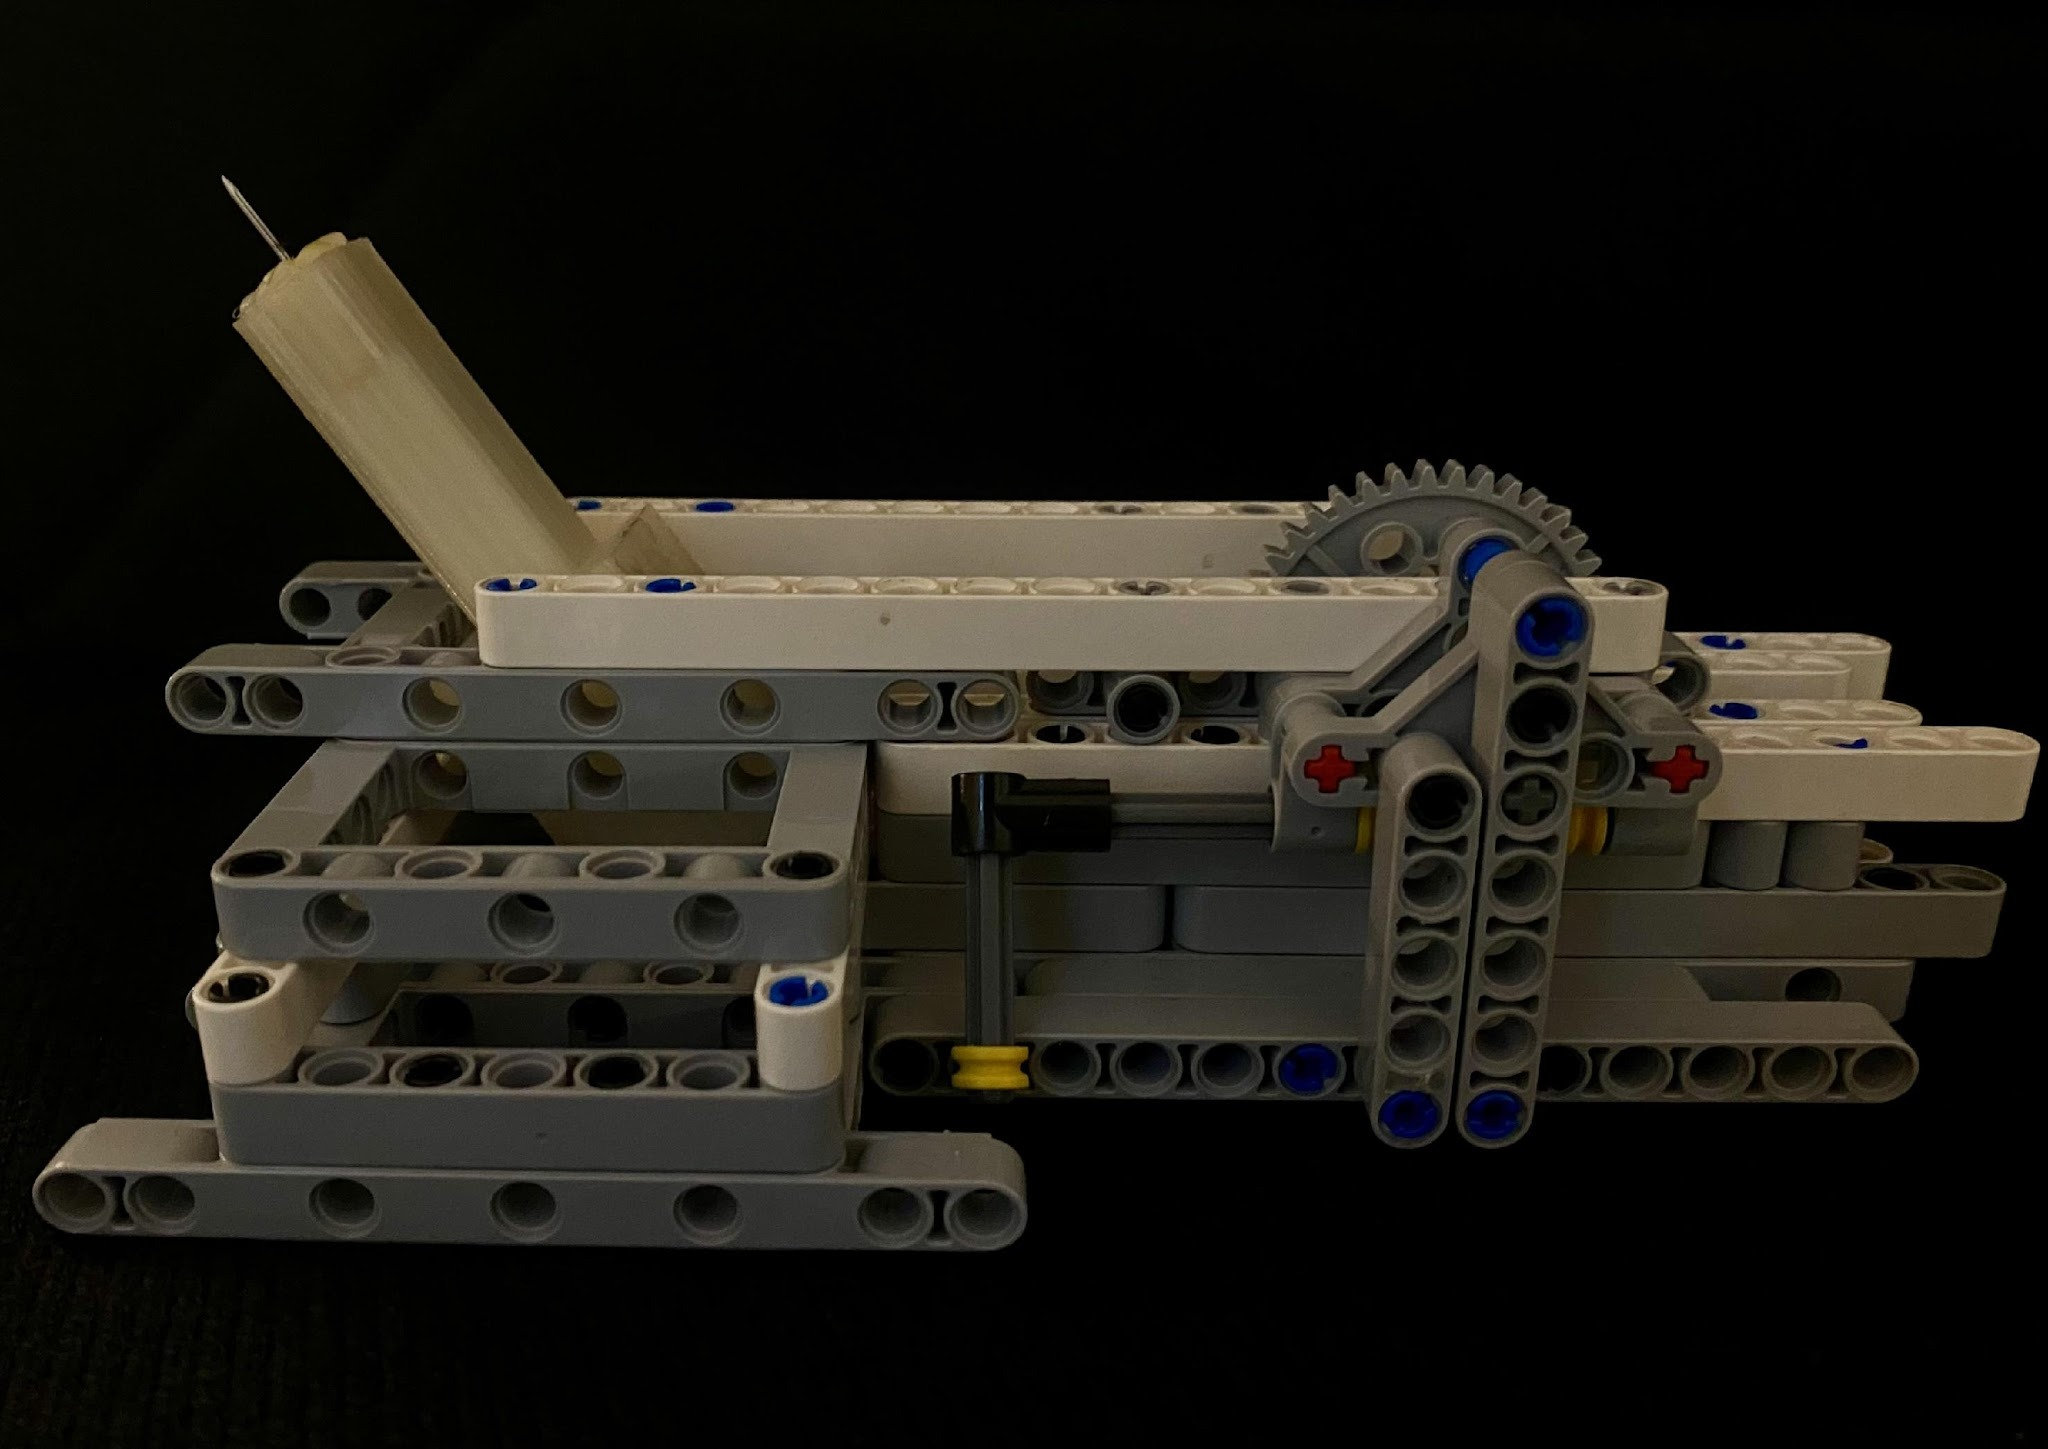
\includegraphics[width=\linewidth,height=2.6cm,keepaspectratio]{launcher_lego.jpg}\caption{}\end{subfigure}\hfill
  \begin{subfigure}[b]{0.49\columnwidth}\centering
    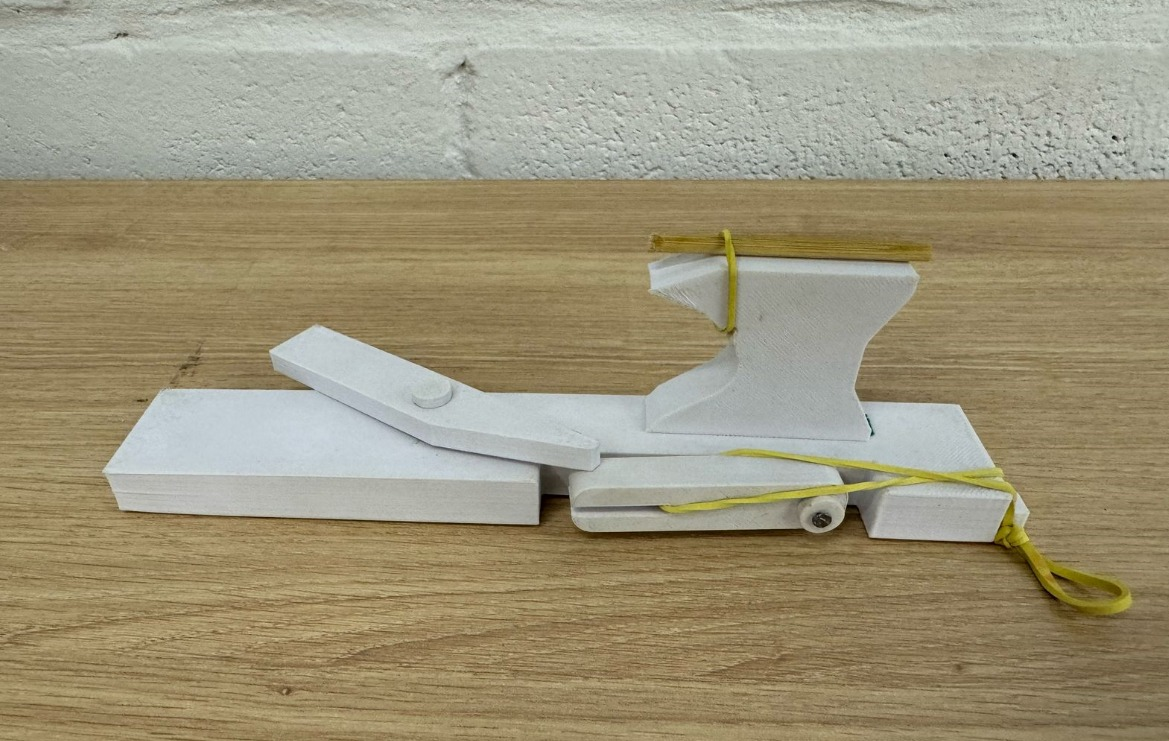
\includegraphics[width=\linewidth,height=2.6cm,keepaspectratio]{launcher_pla.jpg}\caption{}\end{subfigure}\\[2pt]
  \begin{subfigure}[b]{0.62\columnwidth}\centering
    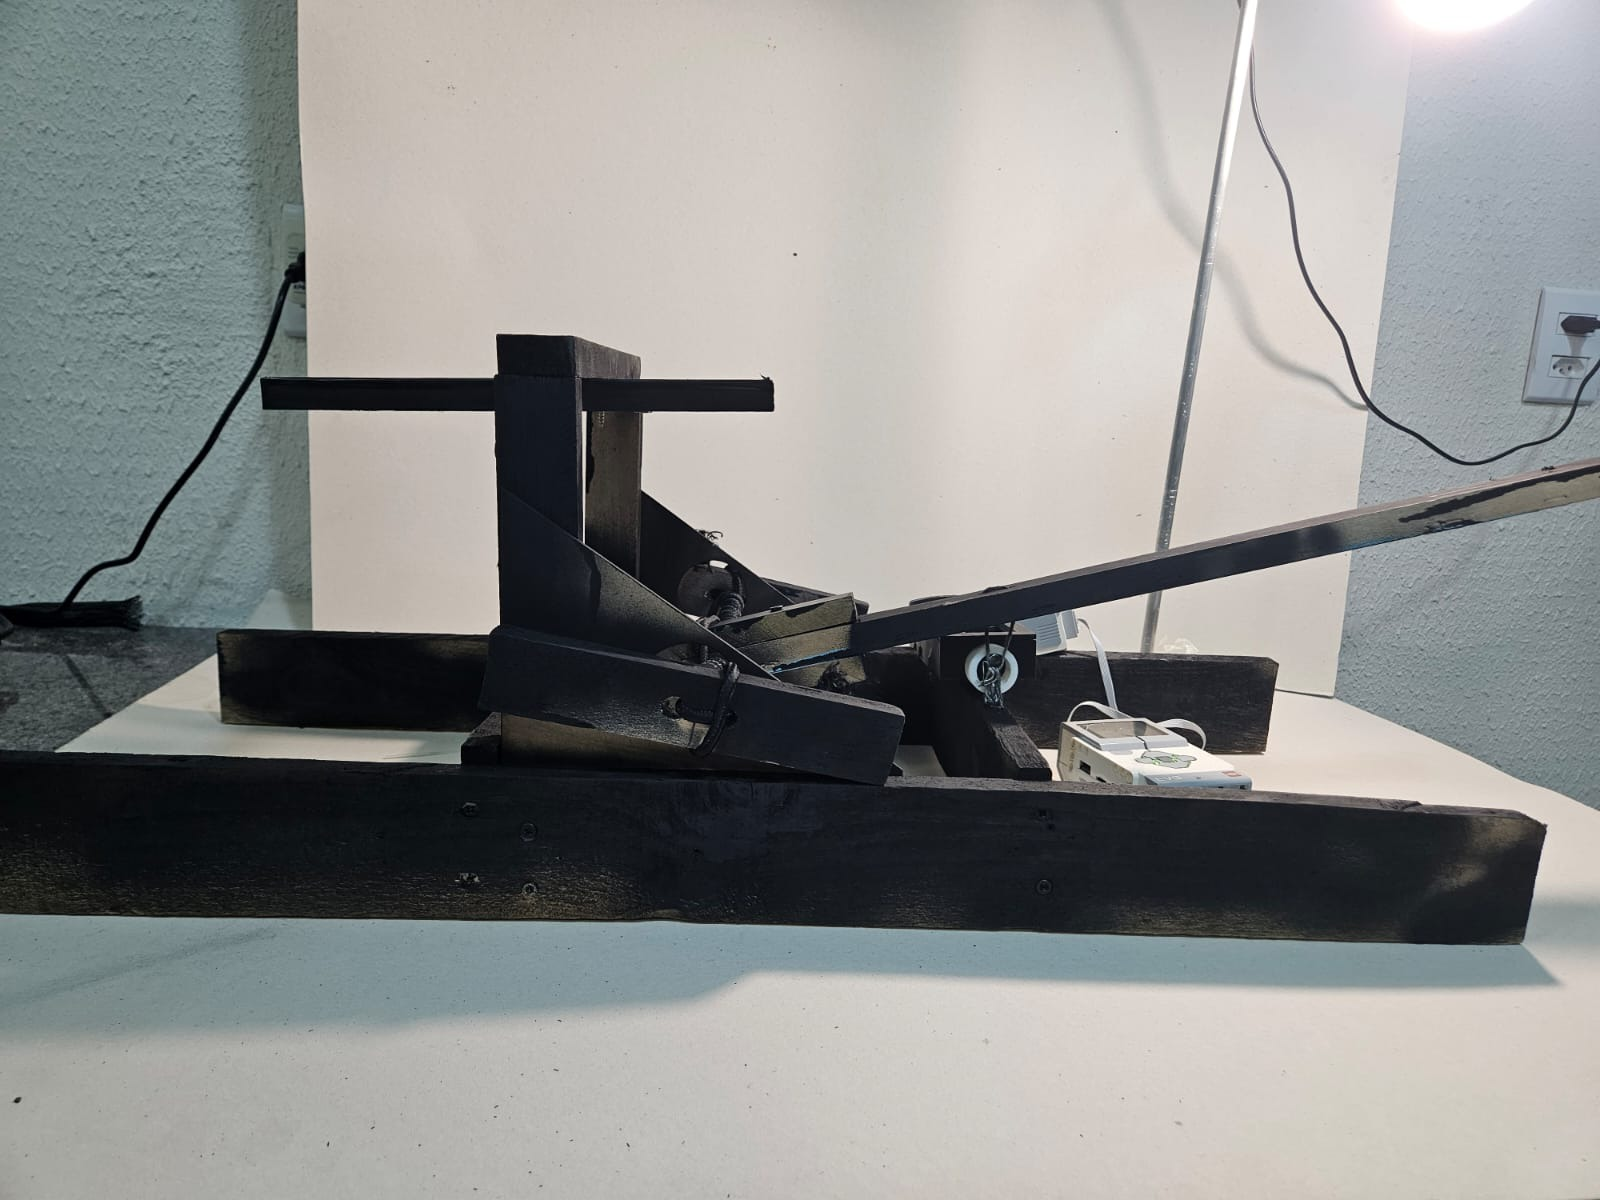
\includegraphics[width=\linewidth,height=4.2cm,keepaspectratio]{launcher_wood.jpg}\caption{}\end{subfigure}\hfill
  \begin{subfigure}[b]{0.36\columnwidth}\centering
    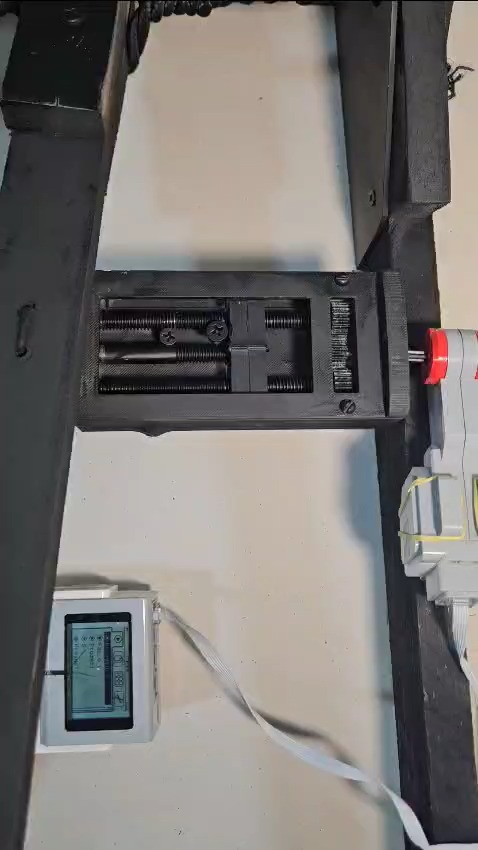
\includegraphics[width=\linewidth,height=4.2cm,keepaspectratio]{launcher_actuator.jpg}\caption{}\end{subfigure}
  \caption{Evolução do lançador. (a)~Lançador de LEGO do Problema~4 do IYPT 2024. (b)~Lançador de PLA impresso em 3D com gatilho lateral, que lançava os bumerangues com força insuficiente. (c)~Catapulta final de madeira com braço acionado por cordas. (d)~Atuador linear controlado pelo EV3, que libera o braço de lançamento.}
  \label{fig:launchers}
\end{figure}

\subsection{Bumerangues}

Construímos três famílias de bumerangues de papel (Fig.~\ref{fig:boomerangs}, Tabela~\ref{tab:boomerangs}): um bumerangue de duas asas feito inteiramente por origami, com arqueamentos antissimétricos; um bumerangue de três asas feito de tiras dobradas e coladas no centro, com arqueamentos simétricos; e bumerangues de quatro asas feitos de origami e cola, com arqueamentos simétricos. Na família de quatro asas, o comprimento do braço foi variado. Os comprimentos foram medidos com resolução de $\pm\SI{0.05}{cm}$.

\begin{table}[b]
  \caption{Geometria dos bumerangues: número de asas $n$, corda $C$ e comprimento do braço $R$. Os comprimentos têm incerteza de $\pm\SI{0.05}{cm}$. O coeficiente de sustentação entra no modelo apenas pelas amplitudes ajustadas da Sec.~\ref{sec:results}.}
  \label{tab:boomerangs}
  \begin{ruledtabular}
  \begin{tabular}{lccc}
    Bumerangue & $n$ & $C$ (cm) & $R$ (cm) \\
    \midrule
    Amarelo (origami)          & 2 & 2,50 & 10,00 \\
    Azul (tiras coladas)       & 3 & 3,00 & 9,40  \\
    Branco, braços longos      & 4 & 2,50 & 7,00  \\
    Branco, braços médios      & 4 & 2,50 & 5,00  \\
    Branco, braços curtos      & 4 & 2,50 & 3,00  \\
  \end{tabular}
  \end{ruledtabular}
\end{table}

\begin{figure*}[t]
  \centering
  \begin{subfigure}[b]{0.27\textwidth}\centering
    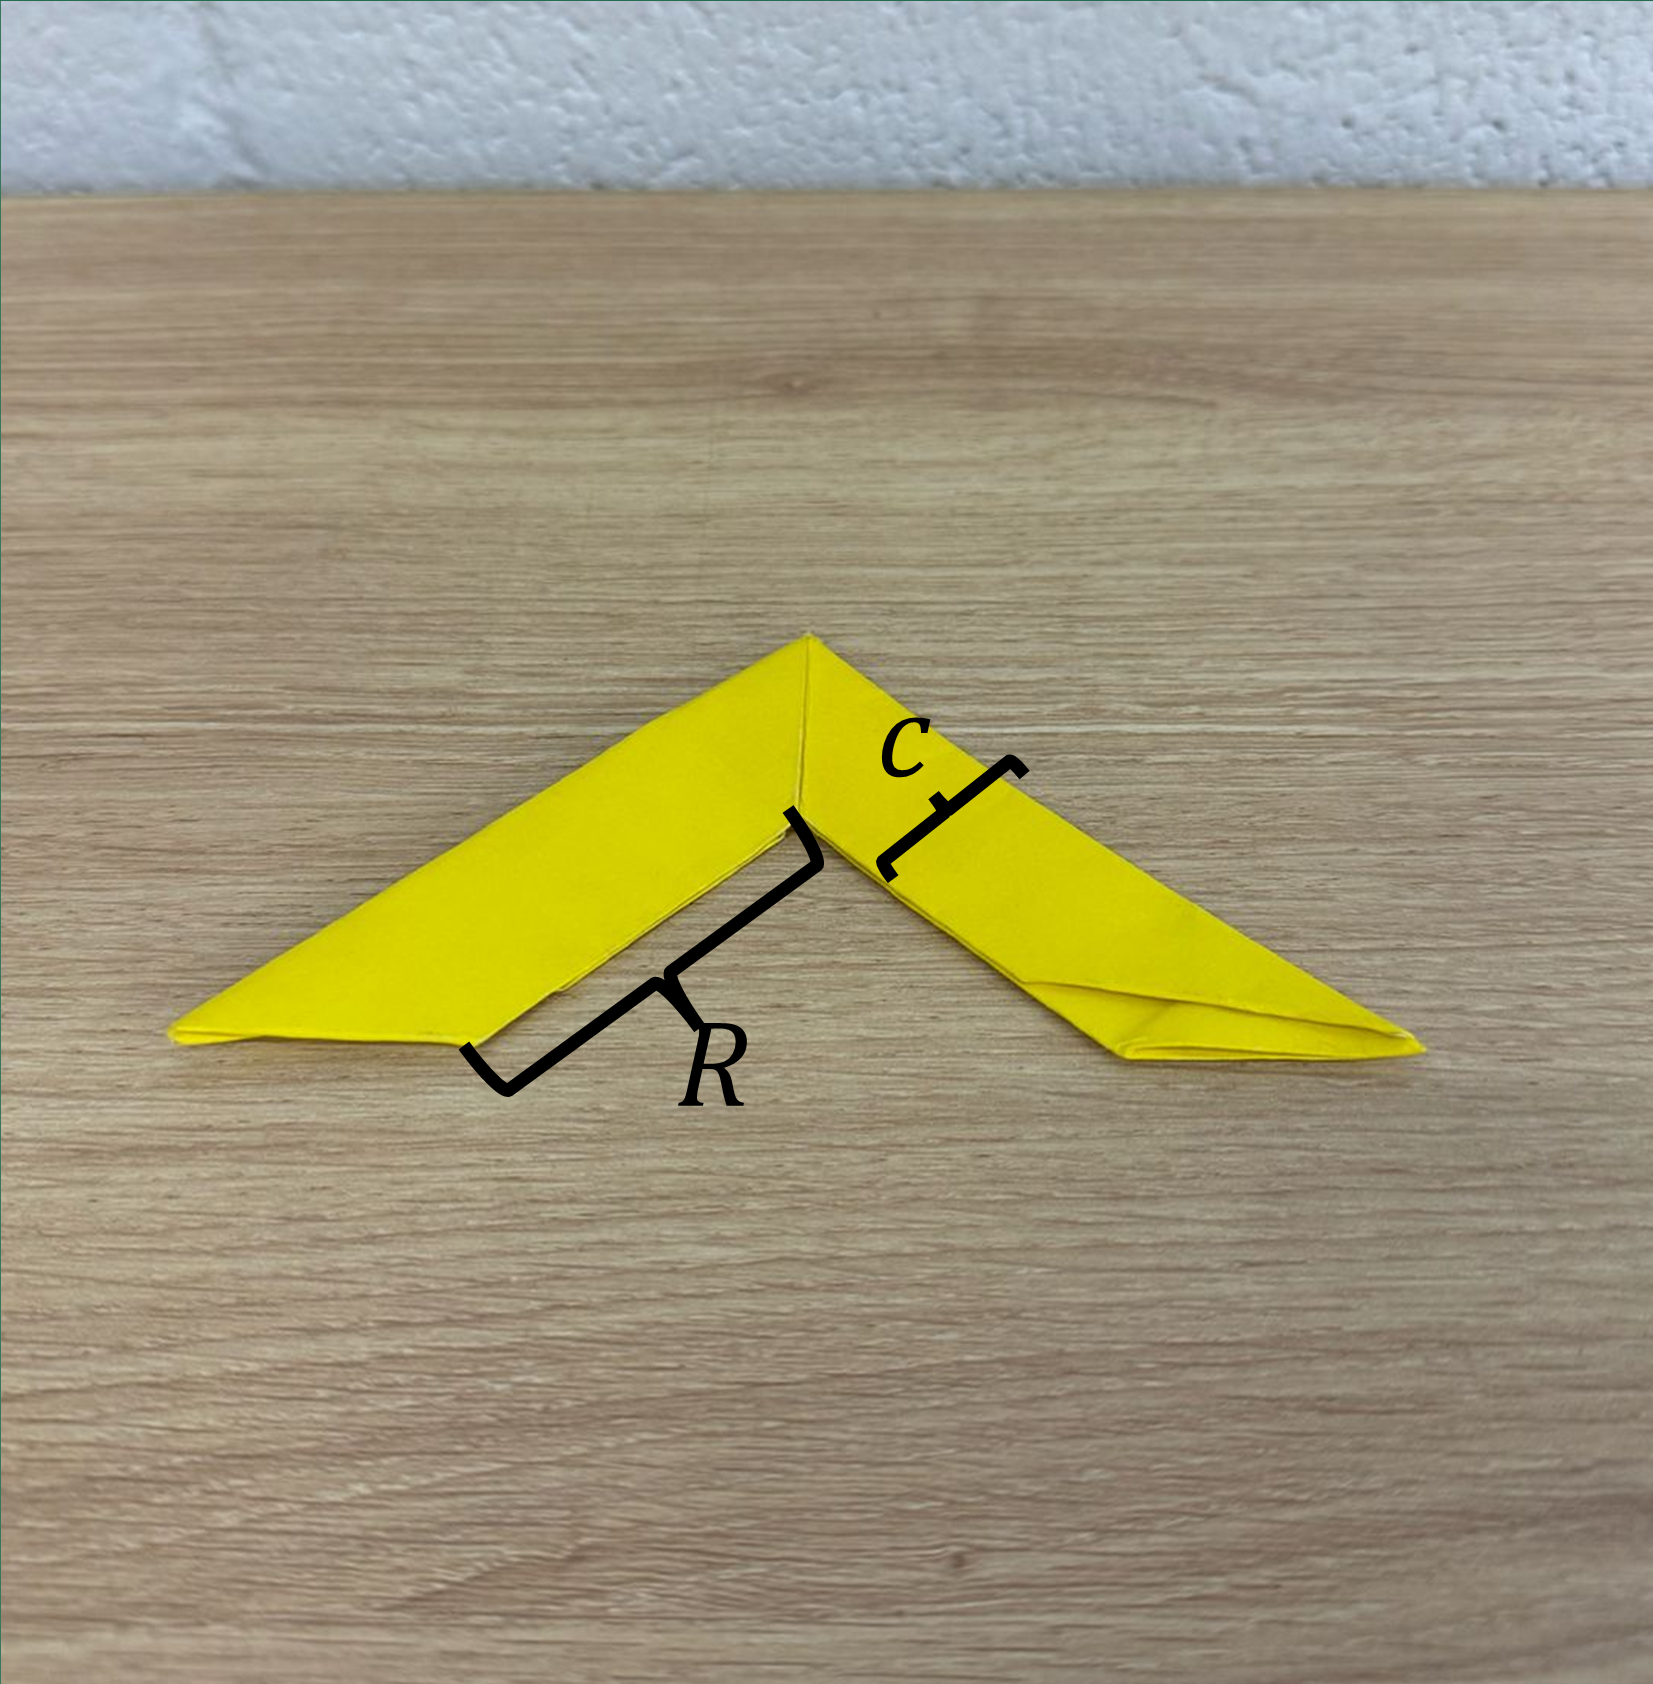
\includegraphics[width=\linewidth]{boomerang_2wing.png}\caption{}\end{subfigure}\hfill
  \begin{subfigure}[b]{0.27\textwidth}\centering
    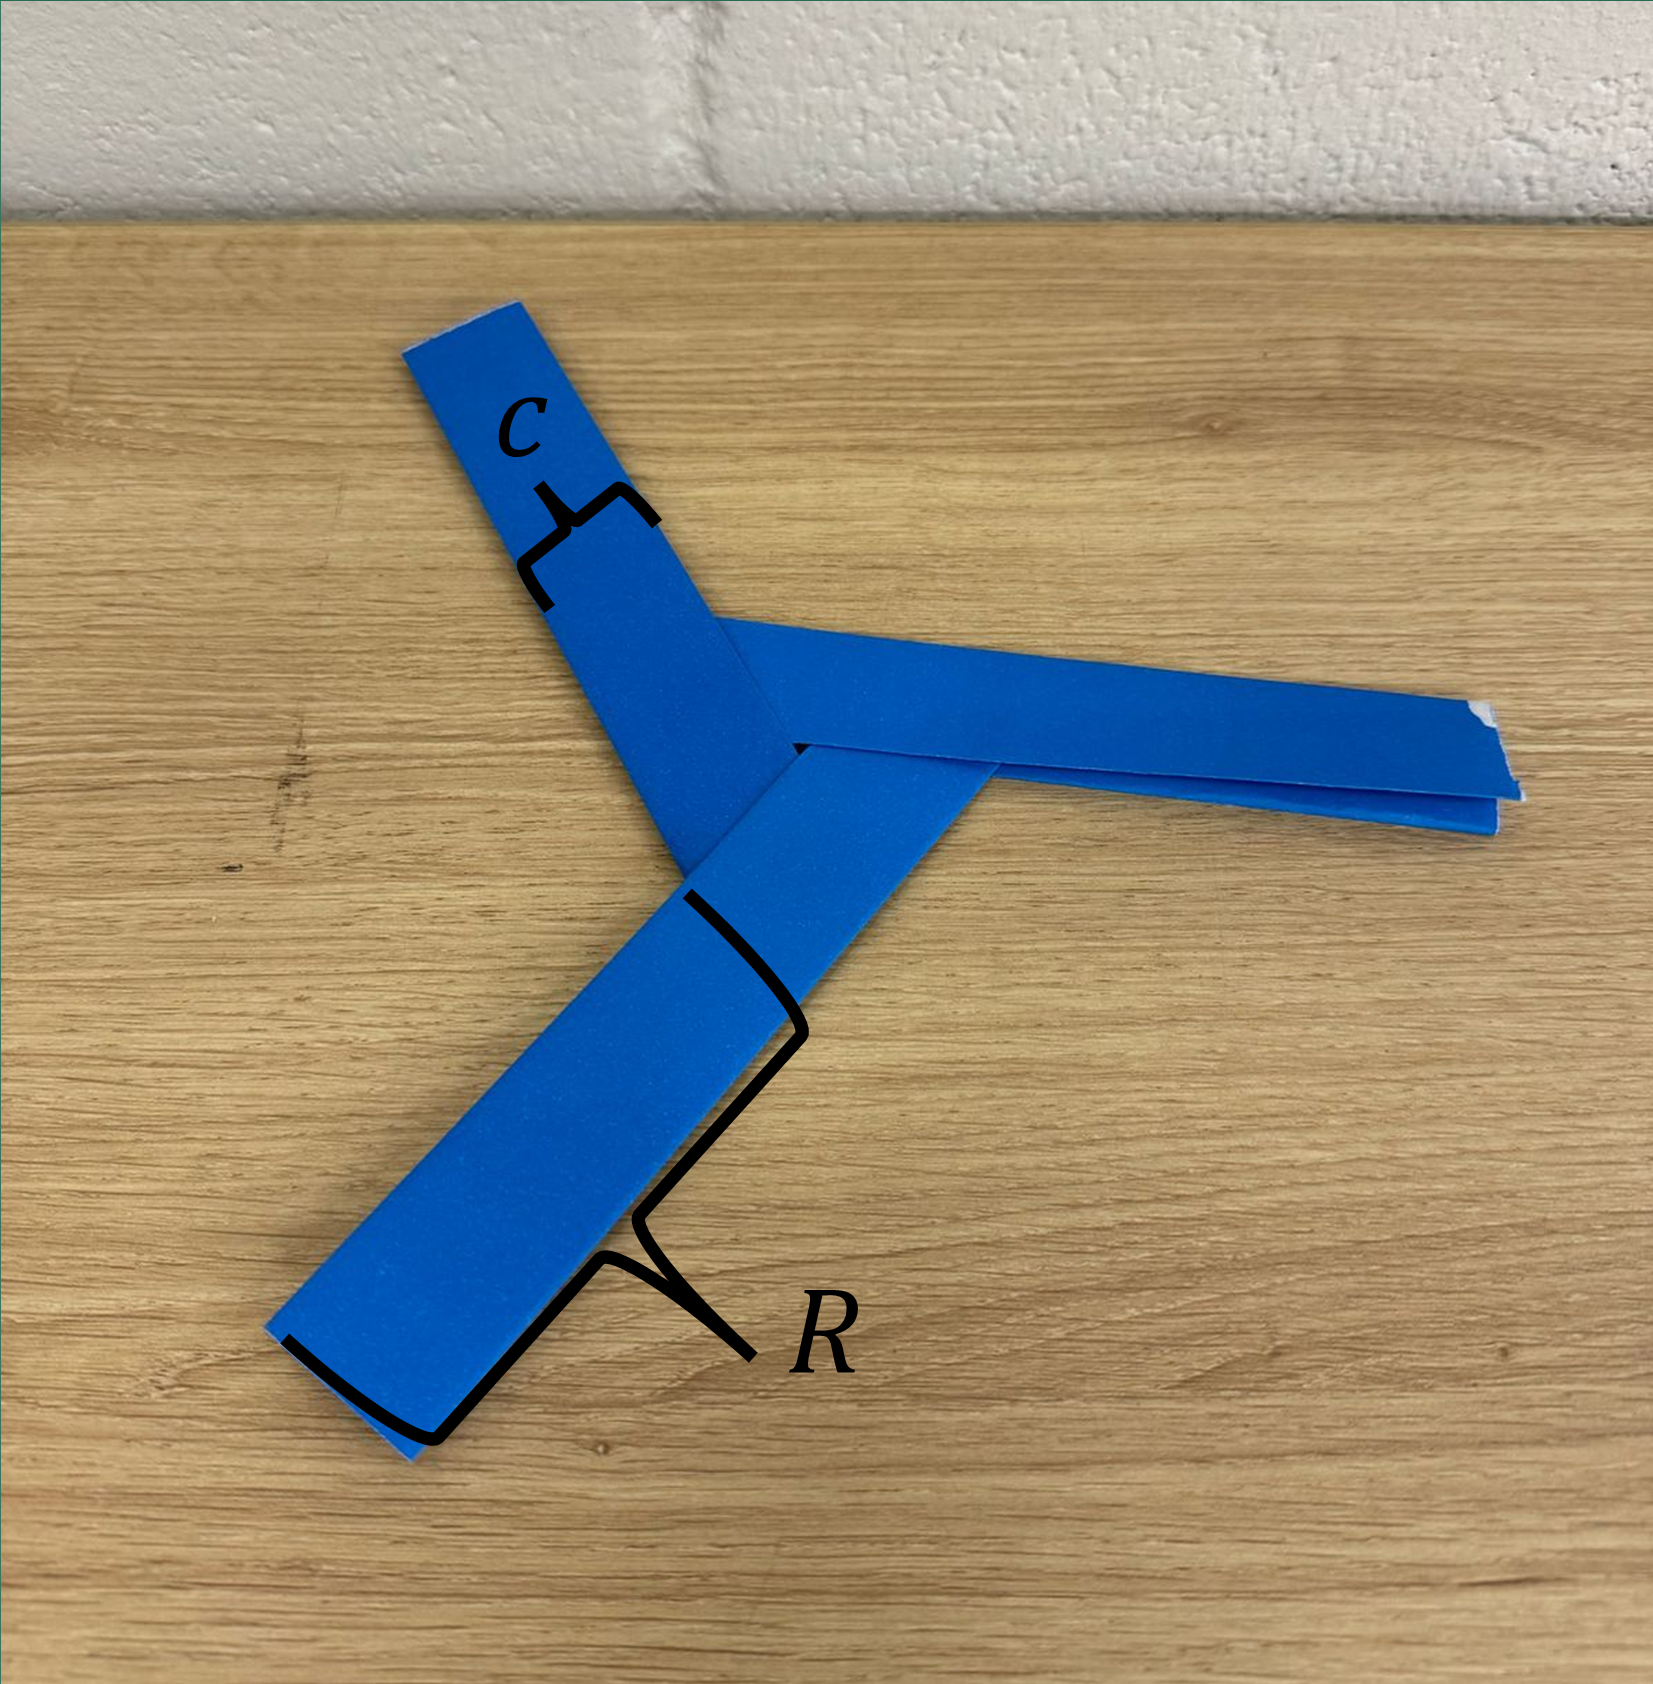
\includegraphics[width=\linewidth]{boomerang_3wing.png}\caption{}\end{subfigure}\hfill
  \begin{subfigure}[b]{0.42\textwidth}\centering
    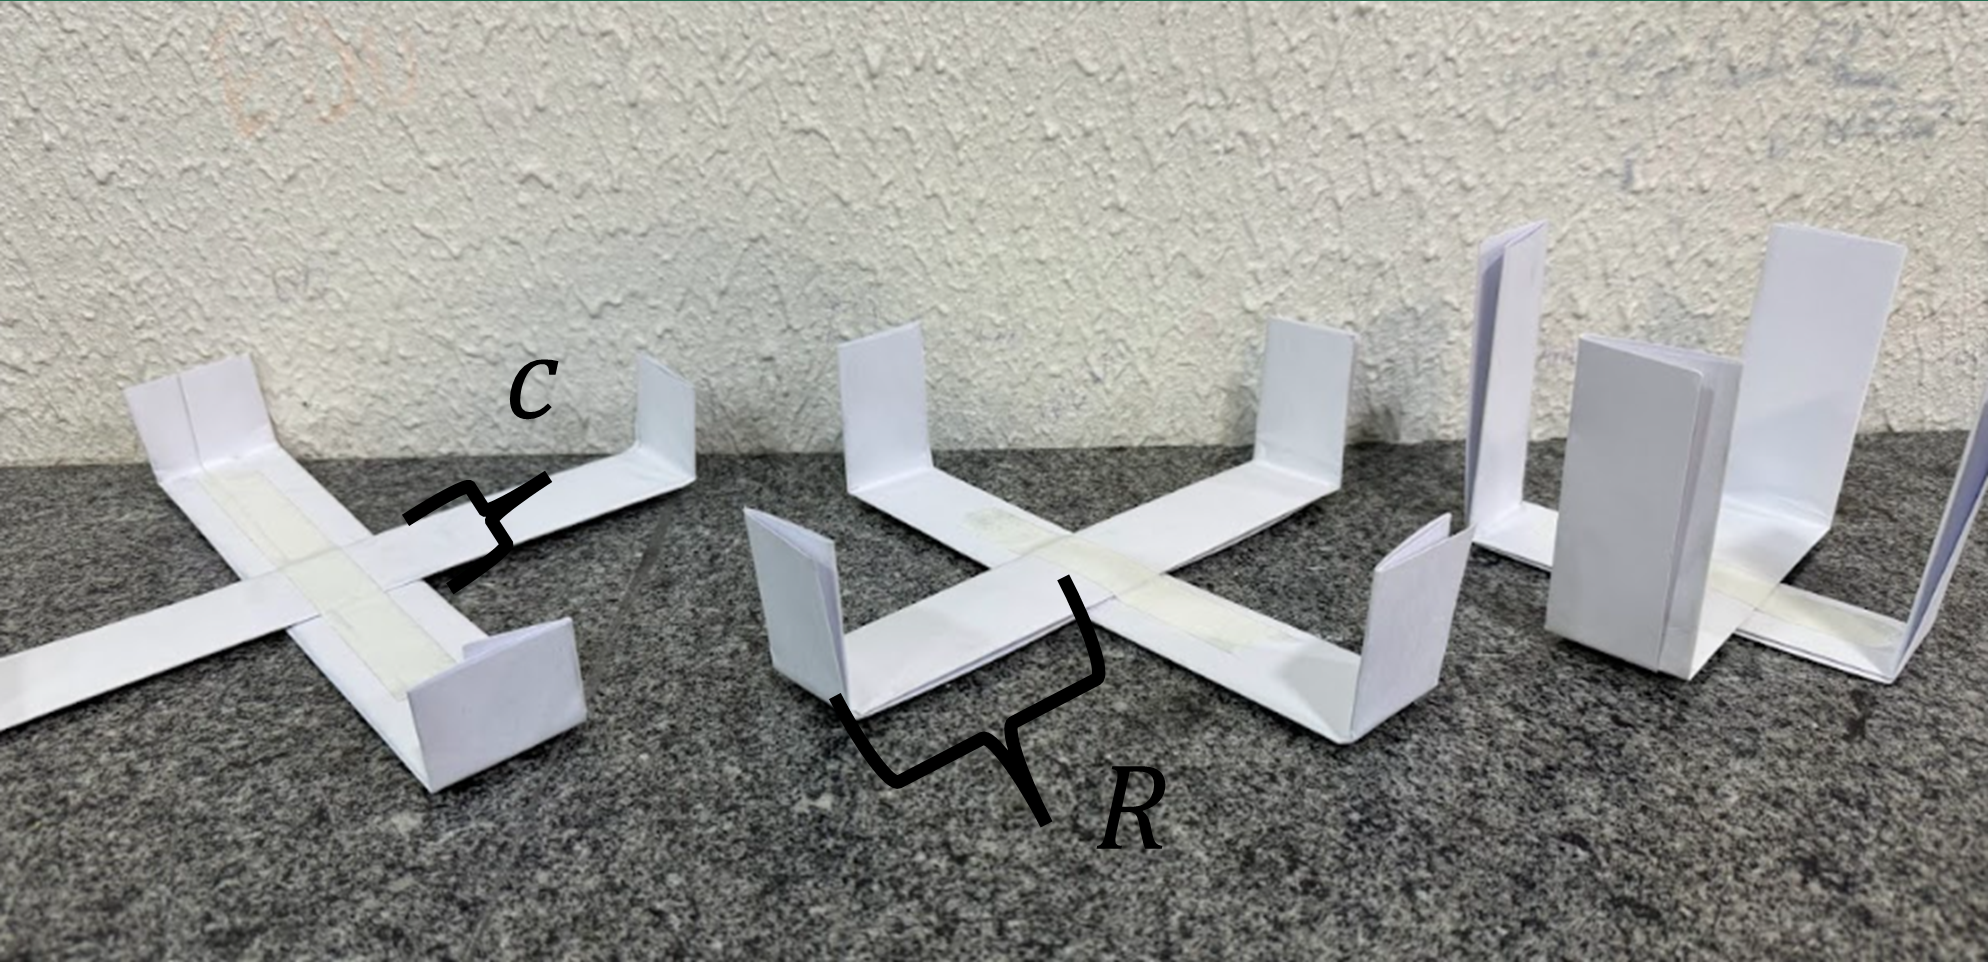
\includegraphics[width=\linewidth]{boomerang_4wing.png}\caption{}\end{subfigure}
  \caption{Bumerangues de papel usados nos experimentos, com a corda $C$ e o comprimento do braço $R$ indicados. (a)~Bumerangue de duas asas em origami. (b)~Bumerangue de três asas. (c)~Bumerangues de quatro asas com diferentes comprimentos de braço.}
  \label{fig:boomerangs}
\end{figure*}

\subsection{Procedimento e grandeza medida}

Os experimentos foram realizados em um ginásio fechado para minimizar o vento [Fig.~\ref{fig:arena}(a)]. A inclinação lateral foi imposta apoiando o lançador sobre uma rampa de madeira. Cada configuração foi repetida sete vezes, e a incerteza estatística foi tomada como o desvio padrão das repetições. Lançamentos em que o bumerangue não se soltou do braço de forma limpa foram descartados. Os voos foram filmados de cima, e a grandeza comparada com a teoria é o desvio lateral do bumerangue em relação à direção inicial de lançamento, como esquematizado na Fig.~\ref{fig:arena}(b).

\begin{figure}[t]
  \centering
  \begin{subfigure}[b]{\columnwidth}\centering
    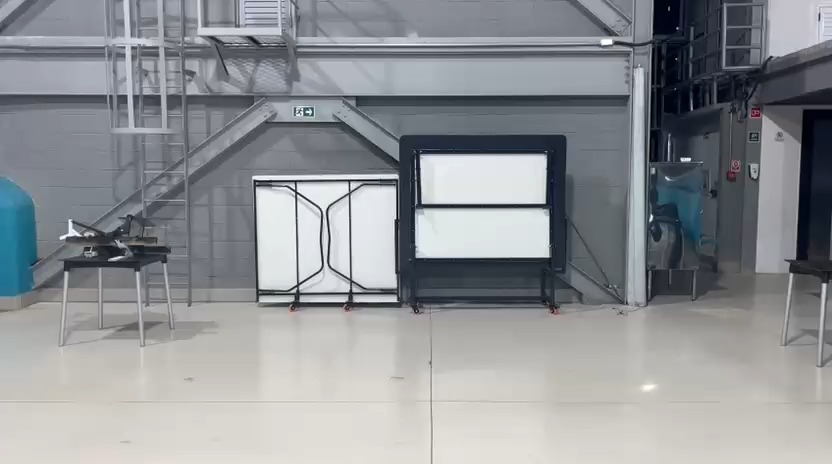
\includegraphics[width=0.9\linewidth]{arena.jpg}\caption{}\end{subfigure}\\[2pt]
  \begin{subfigure}[b]{\columnwidth}\centering
    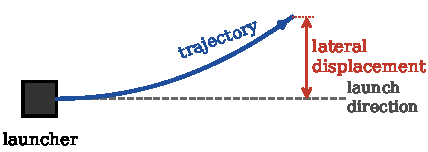
\includegraphics[width=0.9\linewidth]{deviation_schematic.pdf}\caption{}\end{subfigure}
  \caption{(a)~Lançador posicionado no ginásio fechado. (b)~Vista superior de um voo: o desvio lateral usado nas Figs.~\ref{fig:dev_angle} e \ref{fig:dev_spin} é medido perpendicularmente à direção de lançamento (linha tracejada).}
  \label{fig:arena}
\end{figure}

%=====================================================================
\section{Modelo teórico}
\label{sec:theory}
%=====================================================================

Usamos um referencial de laboratório com o eixo $x$ ao longo da velocidade inicial $\vect V_0$, o eixo $z$ vertical e o eixo $y$ horizontal, orientado para o lado em que a trajetória se curva. Para evitar confusão entre momento angular e sustentação, denotamos o momento angular de rotação por $\vect J$, a sustentação por $\vect L$ e o eixo unitário de rotação, normal ao plano do bumerangue, por $\uv s$.

\subsection{Cinemática do elemento de pá}

Considere um elemento de pá de corda $C$ e largura $dr$ à distância $r$ do centro (Fig.~\ref{fig:bet}). As $n$ asas são igualmente espaçadas, de modo que a $i$-ésima asa está no azimute
\begin{equation}
  \psi_i = \psi + \frac{2\pi i}{n}, \qquad i=0,1,\ldots,n-1,
\end{equation}
medido a partir da direção de voo, com $\psi=\omega t$. A velocidade do ar normal ao bordo de ataque do elemento é a soma da velocidade de rotação com a componente da velocidade translacional perpendicular à asa,
\begin{equation}
  U(\psi_i,r) = \omega r + V\sin\psi_i ,
  \label{eq:airspeed}
\end{equation}
maior do lado que avança ($\sin\psi_i>0$) do que do lado que recua. A sustentação do elemento é
\begin{equation}
  dL_i = \tfrac12\,\rho\, U^2(\psi_i,r)\, C_L\, C\, dr,
  \label{eq:dL}
\end{equation}
com $\rho$ a densidade do ar, e o seu momento em torno do eixo de voo tem braço $r\sin\psi_i$. É conveniente introduzir a razão de avanço
\begin{equation}
  \mu \equiv \frac{V}{\omega R},
  \label{eq:mu}
\end{equation}
que compara a translação com a velocidade da ponta da asa. No lado que recua, a velocidade relativa se anula em $r=\mu R\,|\sin\psi_i|$: para $\mu<1$ existe um pequeno disco de escoamento reverso próximo ao centro~\cite{gudem2019}, cuja contribuição para a sustentação é desprezível, pois ali $U^2$ é pequeno.

\begin{figure}[t]
  \centering
  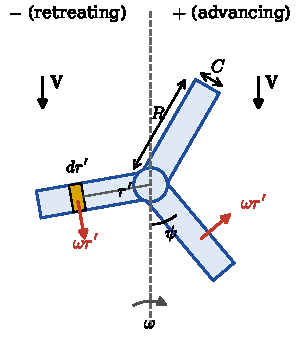
\includegraphics[width=0.85\columnwidth]{bet_geometry.pdf}
  \caption{Geometria do elemento de pá (vista superior) de um bumerangue com braço $R$ e corda $C$ girando a $\omega$. Um elemento de largura $dr'$ no raio $r'$ (sombreado) experimenta a velocidade translacional $\vect V$ e a velocidade de rotação $\omega r'$; as duas se somam do lado que avança ($+$) e se subtraem do lado que recua ($-$) do eixo de movimento (tracejado). $\psi$ é o azimute de uma asa. Adaptado da Ref.~\cite{gudem2019}.}
  \label{fig:bet}
\end{figure}

\subsection{Uma identidade harmônica para rotores de $n$ asas}

A soma sobre as asas pode ser feita exatamente com o seguinte resultado, que é a ortogonalidade das raízes $n$-ésimas da unidade.

\begin{lema}
Para todo inteiro $k$,
\begin{equation}
  \sum_{i=0}^{n-1} e^{\,\mathrm{i}k\psi_i}
  = e^{\,\mathrm{i}k\psi}\sum_{i=0}^{n-1}\left(e^{2\pi\mathrm{i}k/n}\right)^{i}
  = \begin{cases} n\,e^{\,\mathrm{i}k\psi}, & n\mid k,\\[2pt] 0, & n\nmid k.\end{cases}
  \label{eq:lemma}
\end{equation}
\end{lema}

\noindent Portanto, as cargas instantâneas de um rotor de $n$ asas contêm apenas os harmônicos $k\omega$ com $k$ múltiplo de $n$. Escrevendo $\sin^2\psi_i=\tfrac12(1-\cos2\psi_i)$ e $\sin^3\psi_i=\tfrac14(3\sin\psi_i-\sin3\psi_i)$, obtemos
\begin{align}
  \sum_{i}\sin\psi_i &= 0 \quad (n\geq2), \label{eq:S1}\\
  \sum_{i}\sin^2\psi_i &= \frac n2 - \frac{n}{2}\,\delta_{n,2}\cos2\psi, \label{eq:S2}\\
  \sum_{i}\sin^3\psi_i &= -\frac{n}{4}\,\delta_{n,3}\sin3\psi \quad (n\geq2). \label{eq:S3}
\end{align}
Integrando a Eq.~\eqref{eq:dL} ao longo dos braços e somando sobre as asas, a sustentação e o momento de rolamento instantâneos são
\begin{align}
  L(\psi) &= \tfrac12\rho C_LC\sum_{i}\int_0^R U^2\,dr \nonumber\\
  &= \tfrac12\rho C_LC\left[\frac{n\omega^2R^3}{3} + V^2R\sum_i\sin^2\psi_i\right], \label{eq:Linst}\\
  M(\psi) &= \tfrac12\rho C_LC\sum_{i}\sin\psi_i\int_0^R r\,U^2\,dr \nonumber\\
  &= \tfrac12\rho C_LC\bigg[\frac{2\omega VR^3}{3}\sum_i\sin^2\psi_i \nonumber\\
  &\qquad\qquad + \frac{V^2R^2}{2}\sum_i\sin^3\psi_i\bigg], \label{eq:Minst}
\end{align}
onde o termo $\omega^2R^4\sum_i\sin\psi_i/4$ de $M$ se anulou pela Eq.~\eqref{eq:S1}. Daí resulta uma hierarquia notável: para $n\geq4$, a sustentação e o momento são \emph{instantaneamente constantes}; para $n=3$, a sustentação é constante, mas o momento tem uma ondulação de frequência $3\omega$; e para $n=2$ ambos oscilam a $2\omega$. A mesma identidade, aplicada ao tensor de inércia, mostra que para $n\geq3$ os momentos de inércia no plano do bumerangue são iguais, $I_{xx}=I_{yy}=I/2$ (pelo teorema dos eixos perpendiculares), enquanto para $n=2$ eles oscilam a $2\omega$ no referencial do laboratório. O bumerangue de duas asas é, assim, o único cuja dinâmica é parametricamente excitada, o que é consistente com a oscilação observada no início de alguns voos.

\subsection{Médias sobre uma revolução}

As cargas oscilam muito mais depressa do que a trajetória evolui, e por isso as substituímos por suas médias sobre uma revolução completa. Com $\avg{\sum_i\sin^2\psi_i}=n/2$ e $\avg{\sum_i\sin^3\psi_i}=0$ para qualquer $n\geq2$,
\begin{align}
  \avg{L} &= \tfrac12\rho C_L C n\left[\frac{\omega^2R^3}{3}+\frac{V^2R}{2}\right] \nonumber\\
  &= \frac{\rho C_L C n\,\omega^2R^3}{6}\left(1+\frac32\mu^2\right),
  \label{eq:Lavg}\\
  \avg{M} &= \frac{\rho C_L C n\,\omega V R^3}{6}.
  \label{eq:Mavg}
\end{align}
O momento de rolamento é proporcional ao produto $\omega V$: anula-se para um bumerangue que não gira ou que não translada, como esperado da imagem da sustentação assimétrica. Note que a média é feita sobre a revolução completa: cada asa visita alternadamente os lados que avançam e que recuam, e a soma sobre as $n$ asas já inclui ambos os lados.

\subsection{Precessão giroscópica e o mapa exponencial}

A sustentação é perpendicular ao plano do bumerangue, $\avg{\vect L}=\avg{L}\,\uv s$. O momento de rolamento, dirigido ao longo do eixo de voo, é perpendicular ao momento angular $\vect J=I\omega\,\uv s$, onde $I$ é o momento de inércia em torno do eixo de rotação. Ele altera, portanto, a direção de $\vect J$, mas não o seu módulo~\cite{goldstein2002}. No limite giroscópico, $d\vect J/dt=\avg{\vect M}$ dá
\begin{equation}
  \frac{d\uv s}{dt} = \Omega_p\,(\uv v\times\uv s)\times\uv s,
  \qquad
  \Omega_p = \frac{\avg{M}}{I\omega} = \frac{\rho C_L C n R^3 V}{6I},
  \label{eq:sdot}
\end{equation}
com $\uv v=\vect V/V$. Para $\uv v\perp\uv s$, a Eq.~\eqref{eq:sdot} é uma rotação instantânea $d\uv s/dt=\vect\Omega\times\uv s$ com velocidade angular de precessão
\begin{equation}
  \vect\Omega = \Omega_p\,\uv n, \qquad \uv n = \uv v\times\uv s .
  \label{eq:Omegavec}
\end{equation}
A rotação $\omega$ cancela-se da taxa de precessão, mas entra na sustentação, Eq.~\eqref{eq:Lavg}. A aproximação giroscópica exige que a precessão seja lenta frente à rotação própria,
\begin{equation}
  \frac{\Omega_p}{\omega} = \frac{\mu\,\rho C_L S R}{6\kappa\, m} \ll 1,
  \label{eq:gyro}
\end{equation}
onde $S=nCR$ é a área em planta e $I=\kappa mR^2$ define o fator de forma $\kappa$ ($\kappa=1/3$ para braços finos e uniformes). Como $I_{xx}=I_{yy}=I/2$, a nutação ocorre a $2\omega$ e é eliminada pela média.

No lançamento, o bumerangue tem o plano inclinado de $\theta$ em relação à horizontal ($\theta=\SI{90}{\degree}$ corresponde a um plano vertical), de modo que
\begin{equation}
  \uv s_0 = \sin\theta\,\uv y + \cos\theta\,\uv z,
  \qquad
  \uv n = \uv x\times\uv s_0 = -\cos\theta\,\uv y + \sin\theta\,\uv z ,
  \label{eq:axis}
\end{equation}
e $(\uv x,\uv s_0,\uv n)$ é um triedro ortonormal direto [Fig.~\ref{fig:precession}(a)]. Enquanto $\uv n$ permanece fixo, a evolução de qualquer vetor solidário ao plano do bumerangue é dada pelo mapa exponencial do grupo de rotações. Sendo $\mathsf K$ a matriz antissimétrica de $\uv n$, $\mathsf K\vect u=\uv n\times\vect u$, que satisfaz $\mathsf K^3=-\mathsf K$, a série exponencial se reorganiza em
\begin{equation}
  \mathsf R(\Omega) = e^{\Omega\mathsf K}
  = \mathsf{I} + \sin\Omega\,\mathsf K + (1-\cos\Omega)\,\mathsf K^2 ,
  \label{eq:expmap}
\end{equation}
com $\Omega(t)=\int_0^t\Omega_p\,dt'$, que é a fórmula de rotação de Rodrigues~\cite{goldstein2002}:
\begin{equation}
  \mathsf R(\Omega)\vect u = \vect u\cos\Omega + (\uv n\times\vect u)\sin\Omega + \uv n\,(\vect u\cdot\uv n)(1-\cos\Omega).
  \label{eq:rodrigues}
\end{equation}
Como $n_x=0$, a Eq.~\eqref{eq:rodrigues} se escreve, componente a componente,
\begin{widetext}
\begin{equation}
  \mathsf R(\Omega)\vect u =
  \begin{bmatrix}
    u_x\cos\Omega + (n_yu_z - n_zu_y)\sin\Omega \\
    u_y\cos\Omega + n_zu_x\sin\Omega + n_y\,(n_yu_y + n_zu_z)(1-\cos\Omega) \\
    u_z\cos\Omega - n_yu_x\sin\Omega + n_z\,(n_yu_y + n_zu_z)(1-\cos\Omega)
  \end{bmatrix},
  \qquad (n_y,n_z)=(-\cos\theta,\sin\theta).
  \label{eq:rodrigues_components}
\end{equation}
\end{widetext}
Aplicada ao eixo de rotação, com $\uv s_0\cdot\uv n=0$ e $\uv n\times\uv s_0=-\uv x$, ela fornece
\begin{equation}
  \uv s(\Omega) = \uv s_0\cos\Omega - \uv x\sin\Omega
  = \begin{bmatrix} -\sin\Omega \\ \sin\theta\cos\Omega \\ \cos\theta\cos\Omega \end{bmatrix}.
  \label{eq:s_of_Omega}
\end{equation}
A precessão gira o plano do bumerangue e, com ele, a sustentação (Fig.~\ref{fig:lift}); a velocidade só gira porque a sustentação reorientada atua sobre ela.

\begin{figure}[t]
  \centering
  \begin{tikzpicture}[>=stealth,line width=0.8pt,scale=0.95]
    % (a) section seen along x
    \node at (-0.4,2.9) {(a)};
    \draw[->,gray] (-1.9,0) -- (1.9,0) node[right,black] {$y$};
    \draw[->,gray] (0,0) -- (0,2.4) node[above,black] {$z$};
    \draw[gray] (0,0) circle (0.11); \fill[gray] (0,0) circle (0.035);
    \node[below left] at (0,-0.05) {$x$};
    \draw[->,very thick,blue!60!black] (0,0) -- ({1.9*sin(35)},{1.9*cos(35)}) node[above right] {$\uv s_0$};
    \draw[->,very thick,green!45!black] (0,0) -- ({-1.9*cos(35)},{1.9*sin(35)}) node[above left] {$\uv n$};
    \draw[green!45!black] (-0.9,0) arc (180:145:0.9);
    \node[green!45!black] at (-1.15,0.3) {$\theta$};
    \draw[blue!60!black] (0,0.75) arc (90:55:0.75);
    \node[blue!60!black] at (0.3,0.98) {$\theta$};
    % (b) cone
    \begin{scope}[xshift=4.6cm]
      \node at (-1.5,2.9) {(b)};
      \draw[->,very thick,green!45!black] (0,0) -- (0,2.5) node[above] {$\uv n$};
      \draw[dotted,gray,thick] (0,1.6) ellipse (1.3 and 0.32);
      \draw[->,very thick,blue!60!black] (0,0) -- (-1.3,1.6) node[left] {$\uv s$};
      \draw[->,very thick,red!70!black] (0,0) -- (1.25,1.52) node[right] {$\uv s'$};
      \draw[->,thick] (-1.1,1.33) to[bend right=18] node[below,pos=0.5] {$\Omega$} (1.05,1.31);
    \end{scope}
  \end{tikzpicture}
  \caption{(a)~Eixo de precessão $\uv n$ e eixo inicial de rotação $\uv s_0$, vistos ao longo da direção de lançamento $x$ (que sai do papel): ambos estão no plano $yz$, perpendiculares entre si, e inclinados de $\theta$, Eq.~\eqref{eq:axis}. (b)~A precessão de um ângulo $\Omega$ em torno de $\uv n$ gira o eixo de rotação $\uv s$ e, com ele, a sustentação, até $\uv s'$, ao longo de um cone, Eq.~\eqref{eq:rodrigues}.}
  \label{fig:precession}
\end{figure}

\begin{figure}[t]
  \centering
  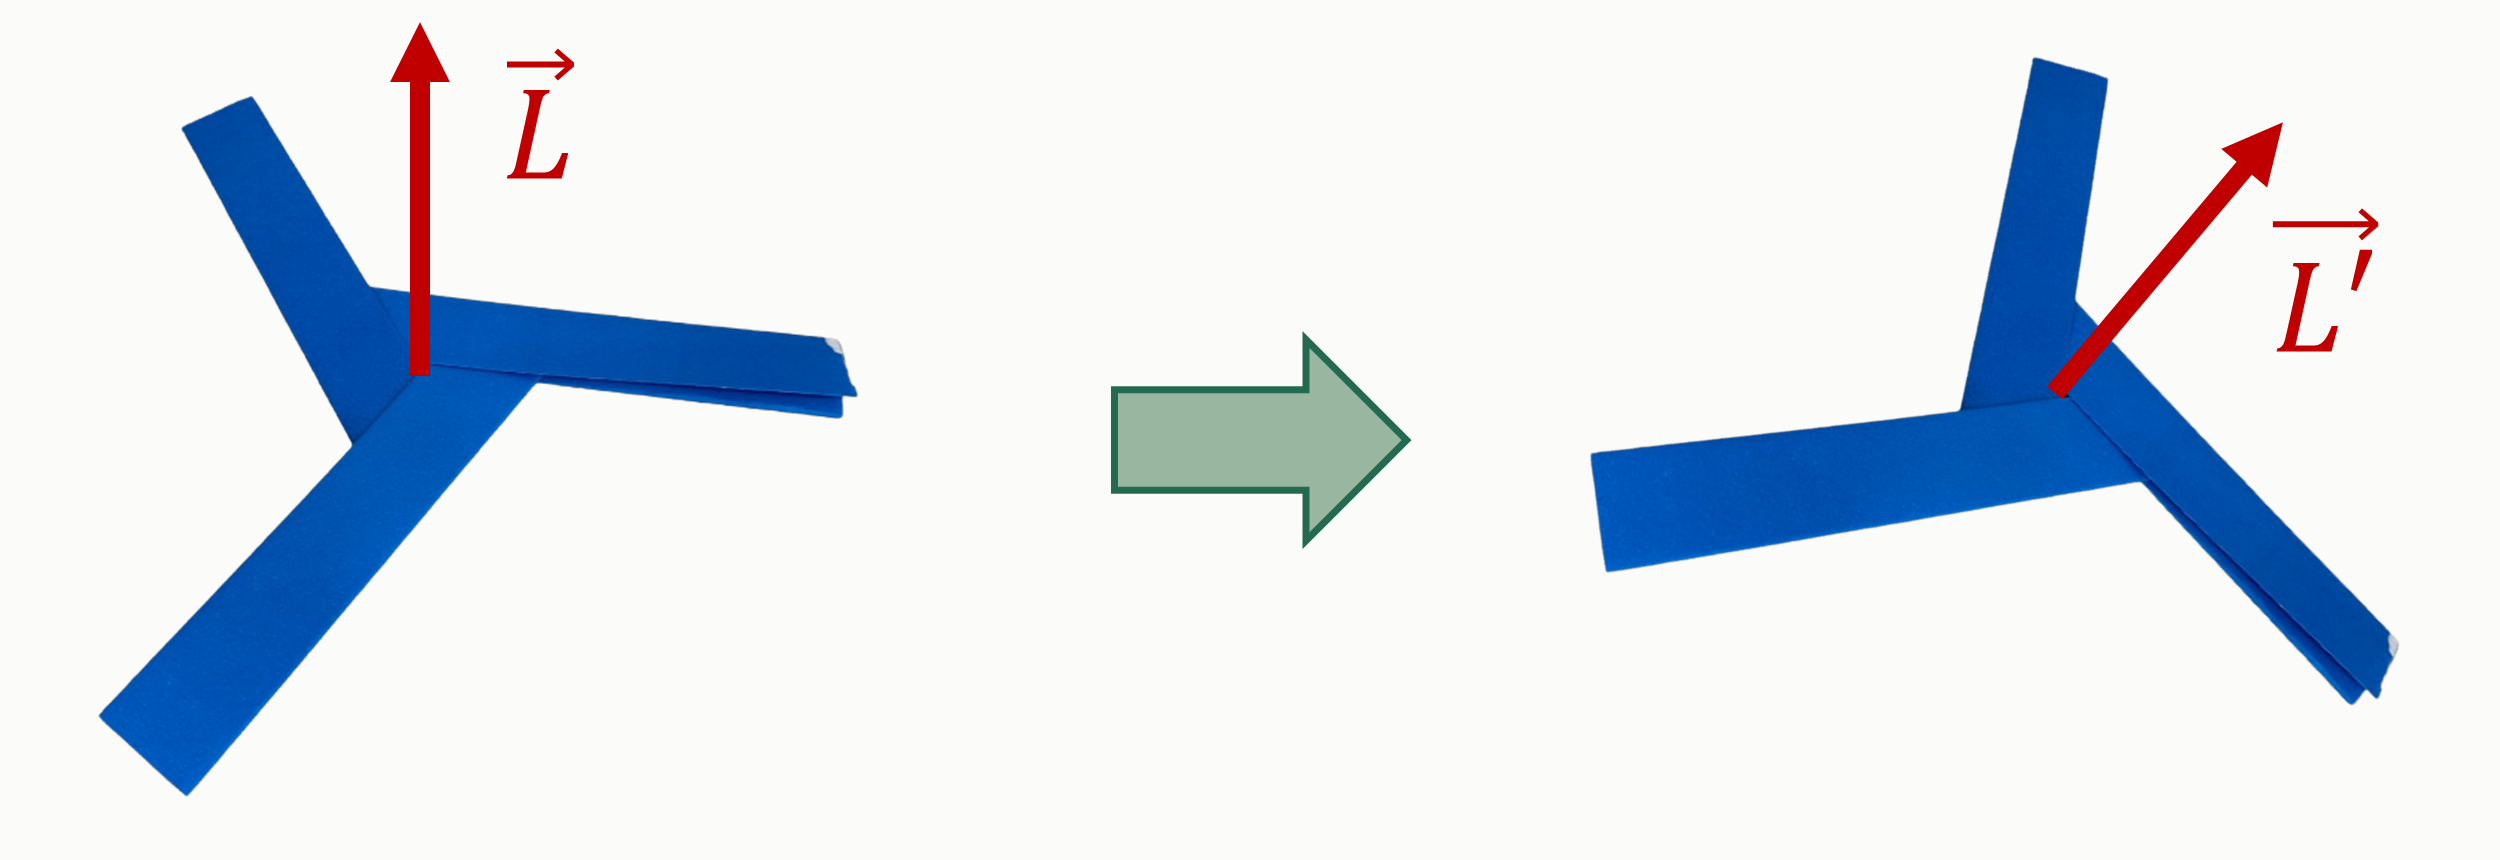
\includegraphics[width=\columnwidth]{lift_reorientation.png}
  \caption{A sustentação $\vect L$ é fixa no referencial do bumerangue; quando o bumerangue precessiona, a sustentação é reorientada para $\vect L'$.}
  \label{fig:lift}
\end{figure}

\subsection{Equações de movimento}

A segunda lei de Newton contém apenas a gravidade e a sustentação média (o arrasto é desprezado). Junto com a Eq.~\eqref{eq:sdot} e a conservação de $|\vect J|$, ela fecha o sistema dinâmico
\begin{equation}
  \left\{
  \begin{aligned}
    m\,\frac{d\vect V}{dt} &= m\vect g + \frac{\rho C_LCn}{2}\left[\frac{\omega^2R^3}{3}+\frac{V^2R}{2}\right]\uv s,\\
    \frac{d\uv s}{dt} &= \frac{\rho C_LCnR^3V}{6I}\,(\uv v\times\uv s)\times\uv s,\\
    \frac{d\omega}{dt} &= 0,
  \end{aligned}
  \right.
  \label{eq:eom}
\end{equation}
com $\vect g=-g\,\uv z$ e as condições iniciais $\vect V(0)=V_0\uv x$, $\uv s(0)=\uv s_0$. A sustentação é perpendicular à velocidade, de modo que, na ausência de gravidade, $V$ é uma constante do movimento.

\subsection{Solução exata: a órbita sincronizada}

O sistema~\eqref{eq:eom} sem gravidade admite uma solução exata em que a velocidade e o eixo de rotação giram juntos, rigidamente, em torno de $\uv n$. Suponha $\uv v(t)=\mathsf R(\Omega)\uv x$ e $\uv s(t)=\mathsf R(\Omega)\uv s_0$ com $\dot\Omega$ constante. Como uma rotação em torno de $\uv n$ preserva $\uv n$, temos $\uv v\times\uv s=\mathsf R(\uv x\times\uv s_0)=\uv n$ em todos os instantes, e o eixo de precessão permanece fixo. Usando $\uv n\times\uv x=\uv s_0$ e $\uv n\times\uv s_0=-\uv x$,
\begin{equation}
  \frac{d\uv v}{dt} = \dot\Omega\,\uv s, \qquad \frac{d\uv s}{dt} = -\dot\Omega\,\uv v .
\end{equation}
A comparação com as Eqs.~\eqref{eq:eom} mostra que esta é uma solução se, e somente se, a taxa de curvatura da trajetória for igual à taxa de precessão,
\begin{equation}
  \frac{\avg{L}}{mV} = \frac{\avg{M}}{I\omega}.
  \label{eq:sync}
\end{equation}
Com as Eqs.~\eqref{eq:Lavg} e \eqref{eq:Mavg}, a condição~\eqref{eq:sync} torna-se $I\omega^2R^2 = V^2\left(mR^2-\tfrac32 I\right)$, isto é, uma razão de avanço universal,
\begin{equation}
  \mu^\ast = \sqrt{\frac{\kappa}{1-\tfrac32\kappa}}
  \;\xrightarrow{\;\kappa=1/3\;}\; \sqrt{\frac23}\approx 0{,}82 ,
  \label{eq:mustar}
\end{equation}
independente da densidade do ar, do coeficiente de sustentação e do número de asas. O raio da órbita sincronizada, $\varrho^\ast=V/\Omega_p$, é
\begin{equation}
  \varrho^\ast = \frac{6I}{\rho C_L nCR^3} = \frac{6\kappa\,m}{\rho C_L S},
  \label{eq:rhostar}
\end{equation}
\emph{independente da velocidade de lançamento}: lançar o bumerangue sincronizado com mais força não aumenta o tamanho do seu círculo, apenas o percorre mais depressa. Esse é o mecanismo pelo qual um bumerangue bem lançado retorna ao lançador. A trajetória é o círculo
\begin{equation}
  \vect r(t) = \varrho^\ast\left[\sin\Omega\,\uv x + (1-\cos\Omega)\,\uv s_0\right], \qquad \Omega = \frac{Vt}{\varrho^\ast},
  \label{eq:circle}
\end{equation}
contido no plano perpendicular a $\uv n$, que está inclinado em relação à horizontal.

\subsection{Traçado no solo e desvio lateral}

Fora da sincronização, o eixo $\uv n$ deixa de ser estritamente fixo, mas a curvatura instantânea da trajetória no plano $(\uv v,\uv s)$ continua sendo $\varrho^{-1}=\avg{L}/(mV^2)$, e a Eq.~\eqref{eq:circle}, com $\varrho^\ast\to\varrho$, descreve o início do voo até segunda ordem em $\Omega$. Projetando-a no plano horizontal, obtemos
\begin{equation}
  x = \varrho\sin\Omega, \qquad y = \varrho\sin\theta\,(1-\cos\Omega),
  \label{eq:ellipse}
\end{equation}
uma elipse de semieixos $\varrho$ e $\varrho\sin\theta$. A gravidade atua apenas ao longo de $z$ e não altera $y$ em primeira ordem. O raio de curvatura do traçado no solo junto ao ponto de lançamento é o do vértice da elipse,
\begin{equation}
  R_c = \frac{\varrho}{\sin\theta} = \frac{mV^2}{\avg{L}\sin\theta},
  \label{eq:Rc}
\end{equation}
e, após uma distância $X\ll R_c$ na direção de lançamento, o desvio lateral é $y\simeq X^2/2R_c$. Com a Eq.~\eqref{eq:Lavg},
\begin{equation}
  y \simeq \frac{X^2\rho C_L C n R\sin\theta}{8m}\left[1+\frac{2}{3\mu^2}\right].
  \label{eq:ylat}
\end{equation}
Supomos que a distância $X$ em que o desvio é lido é aproximadamente a mesma dentro de cada série. A Eq.~\eqref{eq:ylat} faz duas previsões.

\paragraph*{(i) Inclinação.} Para velocidades de lançamento fixas, $y\propto\sin\theta$, com máximo em $\theta=\SI{90}{\degree}$.

\paragraph*{(ii) Rotação.} O lançador fixa a rotação pela posição do ponto de impacto, que divide uma energia de lançamento aproximadamente fixa, $E=\tfrac12mV^2+\tfrac12I\omega^2$, entre translação e rotação. Logo, $V^2=(2E-I\omega^2)/m$ diminui quando a rotação aumenta, e a razão de avanço cai duplamente. Com $f=\omega/2\pi$,
\begin{equation}
  y(f) = a + \frac{b\,f^2}{1-\gamma f^2}, \qquad
  \gamma = \frac{2\pi^2 I}{E}, \qquad
  \frac{b}{a} = \frac{2}{3}\,\frac{mR^2}{I}\,\gamma ,
  \label{eq:yspin}
\end{equation}
que cresce mais rápido que $f^2$ e diverge em $f\to\gamma^{-1/2}$, a rotação em que toda a energia de lançamento seria rotacional. Na linguagem da Eq.~\eqref{eq:ylat}, essa divergência é o limite $\mu\to0$: o bumerangue gira sem transladar, e a curvatura da trajetória cresce sem limite.

%=====================================================================
\section{Resultados e discussão}
\label{sec:results}
%=====================================================================

A Figura~\ref{fig:trajectories} mostra os traçados medidos dos bumerangues de três e de duas asas, junto com círculos tangentes à direção de lançamento ajustados por mínimos quadrados. Os círculos descrevem ambos os traçados com desvio quadrático médio de 1--\SI{2}{cm}, com raios $R_c=\SI{2.03}{m}$ (três asas) e \SI{1.49}{m} (duas asas), como previsto pela Eq.~\eqref{eq:Rc} para um voo com inclinação e velocidade aproximadamente constantes. O traçado do bumerangue de quatro asas sobrepõe-se aos demais no registro original e não pôde ser extraído separadamente.

\begin{figure}[t]
  \centering
  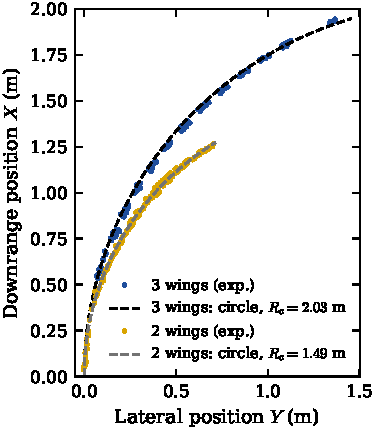
\includegraphics[width=0.85\columnwidth]{trajectories_fit.pdf}
  \caption{Traçados medidos no solo (pontos) dos bumerangues de três e de duas asas e círculos de mínimos quadrados tangentes à direção de lançamento (tracejado), Eq.~\eqref{eq:Rc}. $X$ é a direção de lançamento e $Y$ a coordenada lateral.}
  \label{fig:trajectories}
\end{figure}

O desvio lateral em função da inclinação de lançamento é mostrado na Fig.~\ref{fig:dev_angle}, com ajustes de um parâmetro de $y=A\sin\theta$, Eq.~\eqref{eq:ylat}. Os bumerangues de três e de duas asas seguem a lei em $\sin\theta$ com desvio quadrático médio de \SI{0.1}{cm}, incluindo o máximo em \SI{90}{\degree}. O bumerangue de quatro asas desvia-se até \SI{3}{cm} para grandes inclinações, onde seu desvio satura perto de \SI{21}{cm}. Seus braços curtos e flexíveis são os mais propensos a violar a hipótese de uma asa rígida com inclinação constante.

\begin{figure}[t]
  \centering
  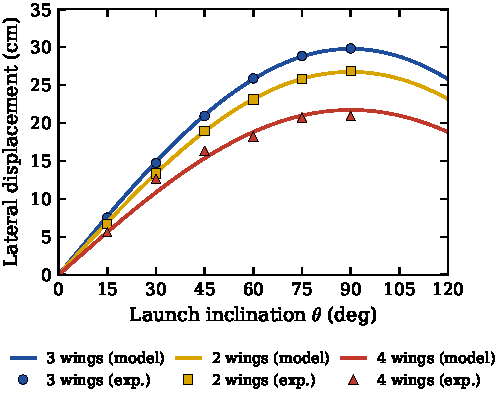
\includegraphics[width=\columnwidth]{deviation_vs_angle_fit.pdf}
  \caption{Desvio lateral em função da inclinação de lançamento $\theta$. Linhas: ajustes de $y=A\sin\theta$, Eq.~\eqref{eq:ylat}; marcadores: experimento (média de sete lançamentos).}
  \label{fig:dev_angle}
\end{figure}

A Figura~\ref{fig:dev_spin} mostra o desvio lateral em função da rotação, com ajustes da Eq.~\eqref{eq:yspin} usando um único valor de $\gamma$ para todos os bumerangues, que foram lançados pela mesma catapulta. O ajuste reproduz o crescimento mais rápido que quadrático para os três bumerangues com desvio quadrático médio de \SI{0.08}{cm}, com $\gamma=\SI{0.048}{s^2}$. Toda a energia de lançamento iria para a rotação em $f=\gamma^{-1/2}\approx\SI{4.6}{rev/s}$, acima da maior rotação utilizada. A razão ajustada entre as amplitudes, $b/a\approx2$--$\SI{2.4}{s^2}$, é, contudo, cerca de 20 vezes maior que o valor permitido pela Eq.~\eqref{eq:yspin} para um bumerangue com $I\approx mR^2/3$. A divisão de energia explica, portanto, a forma da dependência com a rotação, mas não toda a sua intensidade. O ingrediente ausente mais provável é o aumento do tempo de voo em rotações altas, quando a sustentação se aproxima do peso, que a Eq.~\eqref{eq:ylat} não inclui.

\begin{figure}[t]
  \centering
  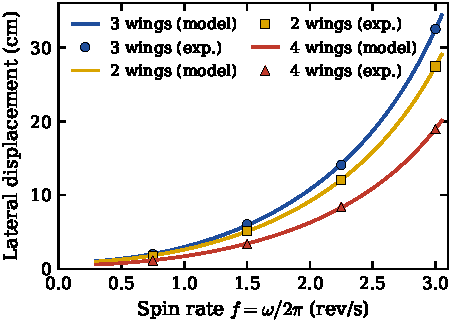
\includegraphics[width=\columnwidth]{deviation_vs_spin_fit.pdf}
  \caption{Desvio lateral em função da rotação. Linhas: ajustes da Eq.~\eqref{eq:yspin} com $\gamma$ comum; marcadores: experimento (média de sete lançamentos).}
  \label{fig:dev_spin}
\end{figure}

\begin{table}[b]
  \caption{Parâmetros ajustados às medidas (incertezas: um desvio padrão do ajuste).}
  \label{tab:fits}
  \begin{ruledtabular}
  \begin{tabular}{lccc}
     & 3 asas & 2 asas & 4 asas \\
    \midrule
    $A$ (cm), Fig.~\ref{fig:dev_angle} & $29{,}8\pm0{,}1$ & $26{,}7\pm0{,}1$ & $21{,}7\pm0{,}5$ \\
    $a$ (cm), Fig.~\ref{fig:dev_spin} & $0{,}87\pm0{,}07$ & $0{,}84\pm0{,}07$ & $0{,}48\pm0{,}06$ \\
    $b$ (cm\,s$^2$), Fig.~\ref{fig:dev_spin} & $2{,}00\pm0{,}02$ & $1{,}68\pm0{,}02$ & $1{,}17\pm0{,}01$ \\
    $\gamma$ (s$^2$), comum & \multicolumn{3}{c}{$0{,}0479\pm0{,}0006$} \\
    $R_c$ (m), Fig.~\ref{fig:trajectories} & $2{,}03$ & $1{,}49$ & -- \\
  \end{tabular}
  \end{ruledtabular}
\end{table}

As principais limitações do modelo são a hipótese de asas rígidas com coeficiente de sustentação constante, questionável para asas de papel que flexionam e para os bumerangues de quatro asas de braços curtos; a omissão do arrasto, que reduz $V$ e $\omega$ ao longo do voo e desloca continuamente a razão de avanço em relação a $\mu^\ast$; a hipótese de escoamento induzido uniforme, que anula o momento de arfagem médio e por isso não descreve o gradual ``deitar'' do plano do bumerangue observado em voos longos~\cite{hess1968}; e o uso de forças médias sobre uma revolução, que não captura a oscilação no início de alguns voos, prevista pela identidade~\eqref{eq:lemma} como exclusiva do rotor de duas asas.

%=====================================================================
\section{Conclusão}
\label{sec:conclusion}
%=====================================================================

Mostramos que uma folha de papel, dobrada e colada em formas de duas, três ou quatro asas, produz um bumerangue que retorna, e explicamos seu movimento pela sustentação assimétrica nas asas que avançam e recuam e pela precessão giroscópica resultante. Uma identidade harmônica sobre as $n$ asas fornece as cargas instantâneas exatas da teoria do elemento de pá e mostra que apenas rotores de $n\geq3$ asas têm sustentação e inércia livres de ondulação. Com médias sobre a revolução completa e a precessão aplicada à direção da sustentação pelo mapa exponencial de $SO(3)$, o modelo forma um sistema dinâmico fechado que admite uma órbita sincronizada exata, com razão de avanço universal $\mu^\ast=\sqrt{2/3}$ e raio independente da velocidade de lançamento. O modelo prevê traçados no solo circulares, um desvio lateral proporcional a $\sin\theta$ e um crescimento mais rápido que quadrático com a rotação, devido à divisão de energia do lançador. As duas primeiras previsões são confirmadas quantitativamente. A terceira reproduz a forma da dependência medida com a rotação, mas subestima sua intensidade, o que aponta o aumento do tempo de voo com a sustentação como o próximo ingrediente a incluir.

\bibliography{references}

\end{document}
